% !TEX encoding = UTF-8
% !TEX TS-program = pdflatex
% !TEX root = ../Tesi.tex
% !TEX spellcheck = it-IT

%************************************************
\chapter{Bitcoin}
\label{bitcoin-chapter}
%************************************************
Questo capitolo ha ls scopo di illustrare al lettore i concetti di \textit{Bitcoin}, \textit{Blockchain} e denaro digitale. Una descrizione più dettagliata la si può trovare nel testo \textit{Mastering Bitcoin} \cite{mastering:andreas}, dal quale sono state prese la maggior parte delle informazioni per la stesura di questo capitolo. Consigliata è anche la lettura del white paper \textit{Bitcoin: A Peer-to-Peer Electronic Cash System} \cite{paper-bitcoin:satoshi}

\section{Introduzione}
Bitcoin è una collezione di concetti e tecnologie che formano le basi per un sistema di denaro digitale. Le unità di valuta si chiamano, appunto, Bitcoin e vengono utilizzate per scambiare valore tra i partecipanti del network Bitcoin. Gli utenti che intendono partecipare a questa rete utilizzeranno un apposito protocollo utilizzando principalmente il canale Internet, anche se sono possibili altri network di trasporto. Sono stati resi disponibili numerosi software open source che implementano l'intero protocollo Bitcoin su di un'ampia gamma di dispositivi digitali, rendendo questa tecnologia facilmente accessibile e flessibile. A differenza delle monete tradizionali, i Bitcoin sono completamente virtuali, la moneta, infatti, è sottintesa nelle transazioni che trasferiscono valuta dal mittente al ricevente. Chi possiede Bitcoin e intende eseguire una transazione, farà uso di chiavi che permettono di avere la prova di essere i proprietari della transazione in oggetto eseguendo lo sblocco della valuta da spendere che verrà quindi trasferita al nuovo ricevente. Il possesso delle chiavi sopraccitate è l'unica prova che dimostra a chi appartiene ogni singolo Bitcoin o frazione di esso, lo smarrimento di queste chiavi implica quindi la perdita dei rispettivi Bitcoin.

Come si sarà intuito, Bitcoin è un sistema distribuito e peer-to-peer, in quanto non ha alcun server centrale o centro di controllo. I Bitcoin sono creati tramite il processo di \textit{mining} che comporta una competizione nel cercare una soluzione di un complesso problema matematico mentre vengono processate le transazioni. Ogni partecipante al network bitcoin che esegue un'istanza completa del protocollo,  può operare come "minatore" utilizzando la potenza di calcolo della propria macchina, verificando e registrando transazioni. In media ogni 10 minuti qualche nodo sarà in grado di validare le transazioni avvenute nei 10 minuti precedenti e questo miner sarà ricompensato con dei bitcoin nuovi di zecca. Il mining Bitcoin decentralizza le emissioni di valuta, attualmente tipiche di una banca centrale, tramite questa competizione globale.

Un importante algoritmo, incorporato all'interno del protocollo Bitcoin, è quello che regola la funzione di minign su tutto il network. La difficoltà della del problema che i miner devono risolvere è infatti calcolata sulla base della potenza computazionale di tutta la rete in modo che si arrivi ad una soluzione ogni 10 minuti circa. Questo protocollo dimezza anche il tasso con cui i nuovi Bitcoin vengono emessi, questo in media ogni 4 anni. Il numero massimo di Bitcoin creati saranno 21 milioni che, con l'andamento attuale si prevede vengano evasi entro l'anno 2140. A causa delle continua diminuzione del tasso di emissione, la valuta Bitcoin è definita deflazionaria, non è soggetta quindi all'inflazione dovuta alla stampa di nuova moneta oltre il limite dato dal tasso di emissione previsto.

\subsection{Storia di Bitcoin}
Bitcoin è stato inventato nel 2008 con la pubblicazione del paper scientifico intitolato \textit{Bitcoin: A Peer-to-Peer Electronic Cash System} \cite{paper-bitcoin:satoshi} scritto da Satoshi Nakamoto. Combinando varie invenzioni scoperte precedentemente, Nakamoto è arrivato alla creazione di un sistema di contante elettronico completamente decentralizzato che non dipende da nessuna autorità centrale, per l'emissione di nuova moneta o per la liquidazione / validazione delle transazioni. Il Problema de \textit{double-spend}, comune nelle valute virtuali, viene quindi risolto. 

La prima implementazione del network Bitcoin nasce nel 2009, in riferimento al Paper pubblicato da Nakamoto \cite{paper-bitcoin:satoshi} e da quel momento fu visto e modificato anche da altri programmatori. Il valore di mercato di Bitcoin al momento è stimato attorno ai 75 miliardi di dollari (USD), che dipende dal tasso di cambio BTC/USD.

Satoshi Nakamoto si ritirò dalla scena pubblica nell'Aprile 2011 lasciando la responsabilità di sviluppo del codice e della gestione del network ad una fiorente comunità di volontari. Nessuno, nè Nakamoto nè chiunque altra persona può esercitare alcun controllo sul sistema Bitcoin, che opera sulla base di principi matematici completamente trasparenti.

\subsubsection{La soluzione ad un Problema Computazionale Distribuito}
L'invenzione di Satoshi Nakamoto è la soluzione pratica ad un problema precedentemente irrisolto, conosciuto come \textit{Byzantine Generals’ Problem}. Questo problema consiste nel tentativo a concordare una linea d'azione condivisa attraverso lo scambio di informazioni su di una rete (network) non affidabile e potenzialmente compromessa. La soluzione proposta da Satoshi Nakamoto usa il concetto di \textit{proof-of-work} per raggiungere il consenso comune senza l'utilizzo di un'autorità centrale. Questo nuovo approccio ha avuto notevoli ripercussioni sulle scienze informatiche che studiano la computazione distribuita soprattutto perché può essere applicata anche ad applicazioni molto diverse da quelle monetarie. L'utilizzo di questa tecnologia può essere utilizzata per arrivare al consenso, su reti decentralizzate, per provare l'equità di elezioni, lotterie, registro di beni, notarizzazione digitale e molto altro.

\subsection*{Tipologie di client Bitcoin}
Per entrare a far parte del network bitcoin e iniziare ad usare la valuta, tutto ciò che tale utente deve fare è scaricare un'applicazione oppure utilizzare una web app disponibile su appositi portali. Dal momento in cui Bitcoin è diventato uno standard sono state sviluppate numerose implementazioni del software del client bitcoin. L'applicazione di riferimento per questi progetti risulta essere \textit{Satoshi client}, progetto open source gestito da un team di sviluppatori derivata dall'iniziale implementazione di Nakamoto. Esistono tre forme principali di client bitcoin:
\begin{enumerate}
	\item \textbf{Full client:} o full node è quel client che salva la storia completa delle transazioni bitcoin e gestisce i wallet dell'utente. Questa tipologia di client è autonomo e non dipende quindi da altri nodi, questo comporta un notevole consumo di memoria occupata appunto dalla \textit{blockchain}\footnote{La blockchain è una tecnologia che permette di creare e gestire un grande database distribuito per la gestione di transazioni condivisibili tra più nodi di una rete. Si tratta di un database strutturato in Blocchi, ognuno contenente più transazioni, che sono tra loro collegati in rete in modo che ogni transazione avviata sulla rete debba essere validata dalla rete stessa nell'analisi di ciascun singolo blocco. La Blockchain risulta così costituita da una catena di blocchi che contengono ciascuno più transazioni.}
	\item \textbf{Lite client:} client più leggero del precedente infatti gestisce i wallet utente localmente ma fa affidamento a server di terze parti per accedere alla rete e alle transizioni bitcoin. Questo client da la possibilità ad un utente di connettersi alla rete bitcoin ma senza dover riservare numerosi GB per la memorizzazione di tutta la blockchain, attualmente sono necessari più di 190 GB.
	\item \textbf{Web client:} classico client al quale si accede tramite un web browser. Questa tipologia di client non salva alcuna informazione in locale infatti anche i wallet utente sono salvati sul server di terze parti che fornisce tale servizio.
\end{enumerate}
La scelta del client bitcoin è molto importante e dipende da quanto controllo si vuole avere sui propri fondi. Un \textit{full client} offrirà all'utente un livello più alto di controllo ed indipendenza, ma fa ricedere il peso dei backup, sicurezza e spazio su disco interamente sulle sue spalle. Al contrario, un \textit{web client}, risulta di più facile utilizzo ma il lato negativo di una simile soluzione è che introduce un rischio di controparte. Infatti la sicurezza e il controllo dei fondi è nelle mani del gestore del servizio. 

\subsection*{Installazione e primo avvio}
Come abbiamo detto in precedenza esistono numerosi software che implementano i client bitcoin, sul testo cui facciamo riferimento \cite{mastering:andreas} viene utilizzato \textit{Multibit}\footnote{Client Bitcoin ora disponibile su multibit.org, questo software non è più supportato pertanto gli sviluppatori consigliano di spostarsi su di un qualsiasi altro client. \cite{multibit-software}}, poi nella successiva versione del libro \textit{Mastering Bitcoin - Programming the Open Blockchain}\cite{mastering2:andreas} viene giustamente abbandonato e sostituito con una più recente applicazione per dispositivi mobili (smartphone android) chiamata \textit{Mycelium}. Dopo l'installazione di questa nuova applicazione, al primo accesso, viene creato in automatico un nuovo wallet nel quale possiamo vedere una sequenza di lettere e numeri, \texttt{1Cdid9KFAaatwczBwBttQcwXYCpvK8h7FK}, troviamo poi anche un \textit{QR Code} che rappresenta la stessa informazione ma che può essere più facilmente scambiata con gli altri utenti tramite l'utilizzo della fotocamera. La stringa di cui stiamo parlando rappresenta appunto l'\textit{Indirizzo Bitcoin}\footnote{Gli indirizzi Bitcoin iniziano sempre con i caratteri 1 o 3, possono essere visti come un indirizzo email con la sola differenza che possono essere creati nuovi indirizzi bitcoin a volontà e ciascuno di essi redirigerà il denaro delle transazioni che lo utilizzano verso lo stesso wallet. Una pratica molto usata per migliorare la privacy sta nel creare nuovi indirizzi per ogni transazione.} dell'utente.

\subsection*{Ottenere i primi Bitcoin}
Il primo e a volte più difficile step è proprio quello di acquisire bitcoin percheé, diversamente dalle altre monete fisiche, non è ancora possibile l'acquisto di bitcoin in banca o nei chioschi dei cambia-valuta. 

Le transazioni bitcoin sono irreversibili a differenza dei ormai classici metodi di pagamento tramite carte di credito / debito, Paypal e trasferimenti bancari che sono reversibili. Nasce perciò il rischio che un qualsiasi venditore di bitcoin venga truffato da utenti che, una volta ricevuti i rispettivi bitcoin, annulli il versamento effettuato tramite i classici pagamenti elettronici. Per mitigare questi fatti un venditore di bitcoin attende qualche giorno / settimana prima di inviare i rispettivi bitcoin, soprattutto se si tratta di un nuovo utente. 

\subsection*{Inviare e Ricevere bitcoin}
Una volta che l'utente ha portato a termine l'installazione del software di gestione del proprio wallet, verrà creato in automatico, oltre all'indirizzo bitcoin, anche una \textit{Private Key} casuale. L'indirizzo bitcoin, infatti, non è altro che un numero casuale che corrisponde ad una chiave privata che l'utente può utilizzare per accedere ai propri fondi. Fino al momento in cui questo indirizzo sarà referenziato come ricevente di un determinato valore in una transazione, inserita nel registro di transazioni bitcoin (\textit{blockchain}), è semplicemente parte del gran numero di indirizzi possibili, ritenuti validi in bitcoin. Quando sarà associato ad una transazione, diventerà parte degli indirizzi conosciuti sul network bitcoin e l'utente cui ci riferiamo, potrà controllare il suo saldo sul registro pubblico.

Per meglio comprendere le prossime azioni, introduciamo due attori Alice e Joe. Alice intende acquistare dei bitcoin da Bob, più precisamente ha intenzione di investirci 10\$. Alice cede una banconota da 10\$ a Joe assieme all'indirizzo bitcoin che le appartiene, in questo modo Joe sarà in grado di inviarle la somma equivalente in bitcoin. A questo punto Joe dovrà scoprire l'attuale tasso di cambio (exchange rate\footnote{Esistono svariate applicazioni che permettono di risalire al tasso di cambio corrente tra cui: Bitcoin Charts, Bitcoin Average, ZeroBlock, Bitcoin Wisdom, ecc\dots}) in modo che possa darle la somma corretta di bitcoin. Attualmente 1 BTC vale 3762,23\$ statunitensi, perciò Joe dovrà versare ad Alice 0,0027 BTC in cambio di 10 dollari (USD). Una volta scoperto il prezzo equo per lo scambio, Joe aprirà la propria applicazione wallet e selezionerà la funzione invio bitcoin dove procederà con l'inserimento dell'indirizzo del destinatario, Alice e della somma di bitcoin da inviare. A questo punto viene costruita una transazione che assegna all'indirizzo di Alice 0,0027 bitcoin, pescando i fondi dal wallet di Joe che ha autorizzato la transazione. Non appena la questa transazione sarà trasmessa attraverso il protocollo peer-to-peer, si propagherà velocemente attraverso il network. In meno di un secondo la maggior parte dei nodi riceveranno tale transazione che verrà processata e successivamente registrata su di un registro globale (blockchain). A questo punto Alice può controllare che tutto sia andato a buon fine accedendo alla propria applicazione wallet che le dovrebbe indicare un saldo di 0,0027 BTC. Se non dovesse trovare i fondi potrebbe significare che la transazione è si stata propagata sulla network ma non è stata ancora inclusa nel registro delle transazioni bitcoin, in questo caso Alice vedrà comunque la transazione di Joe ma con lo stato \textit{Unconfirmed}.

\subsection{Come funziona Bitcoin}
Il sistema bitcoin, al contrario dei sistemi bancari e dei classici sistemi di pagamento, è basato sulla decentralizzazione della fiducia. Invece di un'autorità fiduciaria centrale la fiducia si ottiene come proprietà emergente dall'iterazione tra diversi partecipanti nel network bitcoin. In questo capitolo esamineremo bitcoin eseguendo una singola transazione attraverso tale sistema, osservando quindi come viene gestita la fiducia e come tale transazione viene accettata dal meccanismo di consenso distribuito e venga quindi registrata sulla blockchain, il libro mastro di tutte le transazioni.
\begin{figure}
	\centering 
	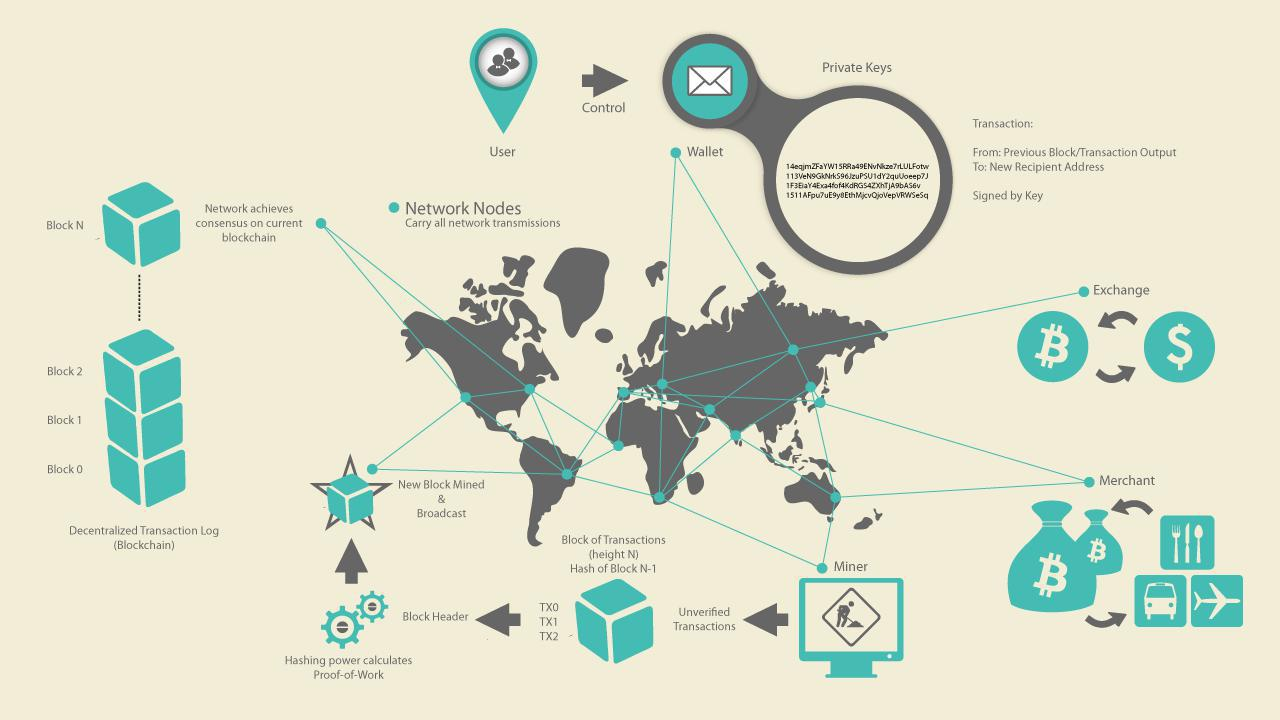
\includegraphics[width=1\columnwidth]{bitcoin} 
	\caption[Panoramica su bitcoin]{Panoramica su bitcoin}
	\label{fig:panoramica-bitcoin} 
\end{figure}
Procedendo nella lettura si troveranno degli esempi di transazioni che sono state effettivamente eseguite sul network, ma che verranno associate a virtuali interazioni tra attori come Alice, Bob e Joe. Per tracciare una transazione in particolare attraverso il network bitcoin e la blockchain, si può utilizzare un blockchain explorer, piattaforma online che opera come un motore di ricerca bitcoin. Questi servizi permettono di cercare per indirizzo, transazione e per blocco e vedere i relativi flussi all'interno di questi.
Tra i Blockchain Explorers più conosciuti troviamo:
\begin{itemize}
	\item Blockchain info https://www.blockchain.com/explorer
	\item Bitcoin Block Explorer https://blockexplorer.com/
	\item Insight https://insight.bitpay.com/
	\item Coinbase https://www.coinbase.com/
\end{itemize} 
Ma vediamo una panoramica del sistema bitcoin, vedi Figura \ref{fig:panoramica-bitcoin}, notiamo che tale sistema è composto di utenti con i propri portafogli (\textit{wallet}) che contengono delle chiavi (\textit{key}), le transazioni si propagano attraverso il network, i miner producono, tramite una gara di computazione, la blockchain del consenso che rappresenta il libro mastro autoritativo di tutte le transazioni.

\subsection{Transazioni Bitcoin}
Una transazione comunica la network che il proprietario di un certo numero di bitcoin ha autorizzato il trasferimento di una parte di essi ad un altro proprietario. Quando tutta l'operazione andrà a buon fine il nuovo proprietario potrà spendere questi bitcoin e di conseguenza spenderli creando una nuova transazione verso un altro utente. Tutto questo genera una catena di passaggi di proprietà.
\begin{figure}
	\centering 
	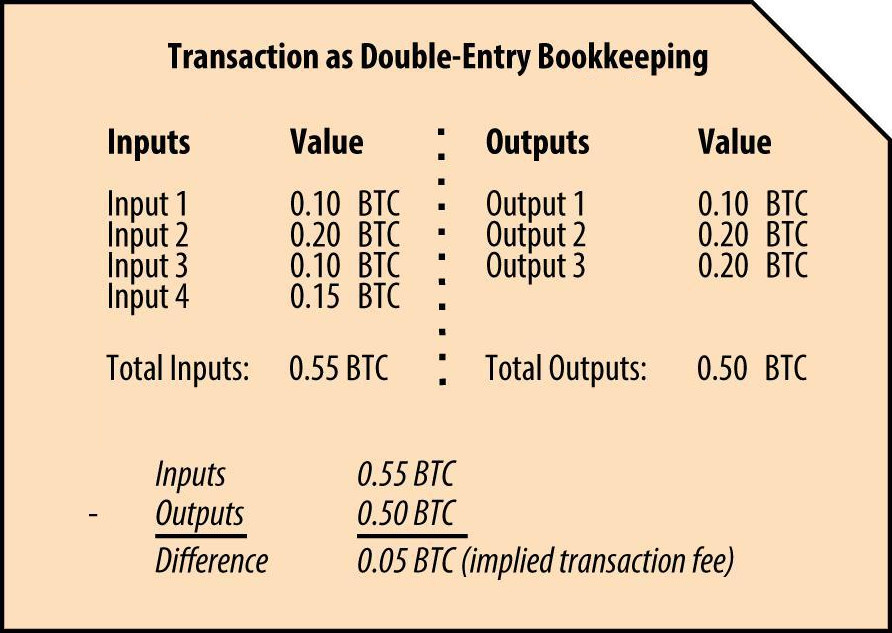
\includegraphics[width=.6\columnwidth]{double-entry-transaction} 
	\caption[Double entry transaction]{Double entry transaction}
	\label{fig:double-entry-transaction} 
\end{figure}
Ogni transazione può contenere uno o più \textit{input}, che sono i debiti verso un account bitcoin. Dall'altro lato della transazione ci sono uno o più \textit{output}, che rappresentano i crediti aggiunti ad un account bitcoin, vedi Figura \ref{fig:double-entry-transaction}. Gli \textit{input} e gli \textit{output} se sommati non totalizzano necessariamente lo stesso risultato. Al contrario, gli \textit{output} risultano poco inferiori rispetto a quello degli \textit{input} e tale differenza rappresenta la \textit{Transaction fee} o Commissione di Transazione sottintesa, che è un piccolo pagamento che il miner ottiene includendo la transazione all'interno del registro. 
\begin{figure}
	\centering 
	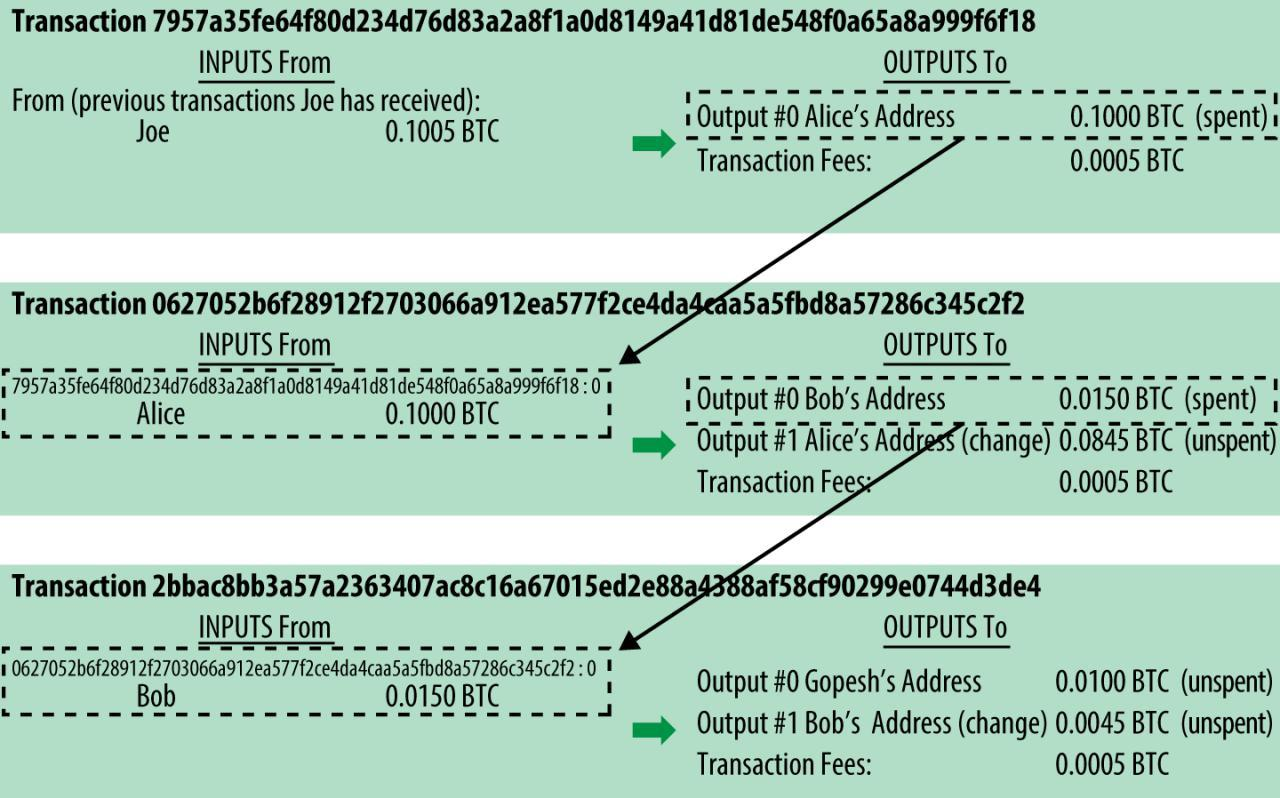
\includegraphics[width=1\columnwidth]{catena-di-transazioni} 
	\caption[Catena di transazioni]{Catena di transazioni}
	\label{fig:catena-di-transazioni} 
\end{figure}
Nella sezione precedente illustravamo come un nuovo potenziale utente potesse ricevere bitcoin in cambio di denaro. Era il caso di Alice e Joe. Tale transazione ha un numero di bitcoin bloccati attraverso la chiave di Alice. Il pagamento che ora Alice intende fare a Bob fa riferimento alla transazione precedente come un input e crea nuovi output per pagare la somma dovuta e per ricevere il resto. Questa rappresenta una vera e propria catena, nella quale gli input dell'ultima transazione corrispondono agli output delle transazioni precedenti. La chiave di alice fornisce la firma che sblocca questi importi in output delle precedenti transazioni, provando a tutta la network che lei è la legittima proprietaria di quei fondi, un esempio di catena la si può vedere in figura \ref{fig:catena-di-transazioni}.

\subsection*{Tipologie di transazione}
Ci sono vari tipi di transazione in base alla quantità di input e output all'interno di essa. Ma vediamoli nel dettaglio:
\begin{itemize}
	\item \textbf{Common Transaction:} la forma più comune di transazione, spesso include un resto e viene ritornato al proprietario originario. Questo tipo di transazione ha un solo input e due output.
	\item \textbf{Aggregating Transaction:} aggrega multipli input in un singolo output. Questa operazione nel mondo reale equivale allo scambiare una pila di monete e banconote per una banconota singola di valore maggiore. Viene comunemete utilizzata per far pulizia da transazioni di valore piccolo, ricevute come resto di numerosi pagamenti precedenti.
	\item \textbf{Distributing Transaction:} transazione che distribuisce un input a più di un outputche rappresentano multipli destinatari. Questo tipo di transazione è talvolta usato dagli esercizi commerciali per distribuire i guadagni, ad esempio quando l'azienda effettua il pagamento degli stipendi ai vari dipendenti.
\end{itemize}

\subsection{Costruire una transazione}
L'applicazione wallet di Alice contiene un'apposita logica che fa in modo di selezionare gli appropriati input e output per costruire una transazione secondo le specifiche imposte da Alice che dovrà solamente specificare una destinazione e l'importo desiderato, il resto viene fatto dall'applicazione.

\subsection*{Ottenere gli input giusti}
L'applicazione wallet di alice deve essere in grado di comporre una transazione inserendo gli input, intesi come frammenti di bitcoin che le appartengono, del valore che intende inviare come pagamento a Bob.Le varie tecniche per fare ciò dipendono dalla tipologia di client che Alice possiede oppure dal fatto che tenga aggiornato un'indice completo dei propri unspent output di ogni transazione nella blockchain. Nel caso Alice non mantenga aggiornato un indice del genere, ha comunque la possibilità di ricavare tale insieme di unspent bitcoin tramite svariate API anche utilizzando un semplice client HTTP. 
\begin{lstlisting}
{
 "unspent_outputs":[
  {
   "tx_hash":"186f9f998a5...2836dd734d2804fe65fa35779",
   "tx_index":104810202,
   "tx_output_n": 0,
   "script":"76a9147f9b1a7fb68d60c536c2fd8...f3cc025a888ac",
   "value": 10000000,
   "value_hex": "00989680",
   "confirmations":0
  }
 ]
}
\end{lstlisting}
Quella mostrata nel riquadro qui sopra risulta la risposta ad una possibile richiesta da parte di Alice che contiene un unspent output. Viene riportata anche la referenza alla transazione nella quale questo unspent bitcoin è contenuto e il relativo valore in bitcoin, 10 milioni, equivalente a 0.10 BTC. Con questa informazione il wallet di Alice potrà costruire una transazione utilizzando questo valere come input e quindi trasferire quel valore all'indirizzo del nuovo proprietario.\\
\textbf{NB:} In questo caso il wallet di Alice dispone di un unspent output con abbastanza bitcoin che riesce a coprire la sua spesa. In alcuni casi può succedere di non disporre di un unico unspent output che riesce a coprire il debito da saldare. In questi casi si dovrà procedere con l'inserimento all'interno della transazione di altri unspent output fino a coprire la spesa da sostenere. In ogni caso Alice dovrà attendersi del resto ma quello lo vedremo nella prossima sezione.

\subsection*{Creare gli output}
La transazione che sta per creare Alice, oltre agli input, include almeno un nuovo output che sarà creato facendo in modo che possa essere riscattato solamente dal legittimo proprietario, in questo caso Bob. Tutto ciò è possibile creando l'output in questione sotto forma di script che creerà un blocco sul valore e potrà essere riscattato solamente da chi sottoporrà una soluzione, in questo caso ci si aspetta la firma della chiave corrispondente all'indirizzo pubblico di Bob. Solo il wallet di Bob potrà presentare una simile firma dal momento che è il creatore di tale chiave pubblica. 
Questa transazione inoltre dovrà includere un'ulteriore output, dal momento in cui i fondi di Alice sono nella forma di un output di 0.10 BTC, un valore elevato se paragonato al pagamento di una cifra d'esempio di 0.015 BTC. In questo caso ad alice spetterebbero 0.085 BTC di resto. Questa cifra andrà rappresenta il secondo output della transazione che sarà indirizzato ad Alice.
Infine, per fare in modo che il network processi la transazione in tempi ragionevoli, l'applicazione wallet di Alice aggiungerà una piccola commissione di transazione (fee). Questa non viene esplicitata nella transazione ma è data dalla differenza tra gli input e gli output, quindi se Alice imposterà l'output resto a 0.0845 BTC avanzeranno 0.0005 BTC. Questa transaction fee sarà recuperata dal miner come commissione per aver incluso la transazione all'interno di un blocco e averla scritta all'interno del registro blockchain. La transazione risultante, una volta confermata ed inviata sul network, può essere vista utilizzando un'applicazione web del tipo blockchain explorer, vedi Figura \ref{fig:transazione-alice-bob}.
\begin{figure}
	\centering 
	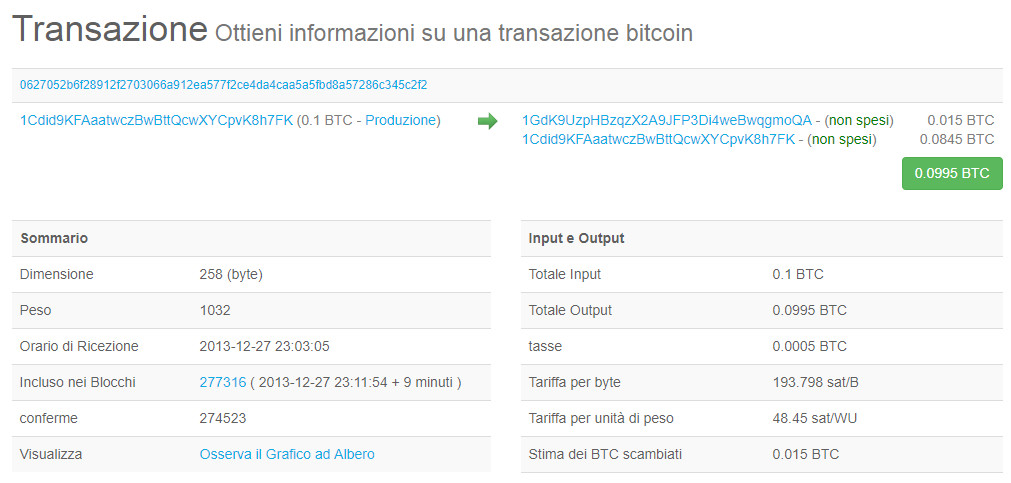
\includegraphics[width=1\columnwidth]{transazione-alice-bob} 
	\caption[Transazionte tra Alice e Bob]{Transazionte tra Alice e Bob}
	\label{fig:transazione-alice-bob} 
\end{figure}

\subsection*{Aggiungere la transazione al Ledger}
In questo momento la transazione tra Alice e Bob viene inviata al network e, come vediamo in Figura \ref{fig:transazione-alice-bob}, risulta avere una grandezza di 258 byte. Come abbiamo visto, all'interno di essa troviamo tutto il necessario per confermare la proprietà dei fondi e assegnare loro nuovi proprietari. La presenza di tutte informazioni danno modo a Bob di verificare fin da subito la transazione controllando che gli input utilizzati corrispondano a precedenti unspent output oltre a verificare che gli importi, comprese le fee, siano adeguati. Bob dovrà aspettare in media 10 minuti per vedere la propria transazione come \textit{confermata}, quindi inserita all'interno del Ledger.

\section{Il Mining di Bitcoin}
Una transazione non entra a far parte del libro mastro condiviso (blockchain) fino a che non viene verificata ed inclusa in un blocco da un processo chiamato \textit{mining}. Il processo di mining in bitcoin serve a due scopi:
\begin{itemize}
	\item Il processo di mining genera nuovi bitcoin per ogni blocco. La quantità di bitcoin creata per ogni blocco è fissa e diminuisce col passare degli anni.
	\item Il mining genera fiducia assicurando che le transazioni siano confermate solo se è stata usata una sufficiente potenza di calcolo. Il problema da risolvere è basato su di un hash crittografico.
\end{itemize}
Ogni 10 minuti un miner entra a far parte di una competizione globale tra miners, alla ricerca di una soluzione per un blocco di transazioni. Trovare tale soluzione, chiamata \textit{proof-of-work}, richiede decine di miliardi di operazioni hash al secondo in tutta la rete bitcoin. L’algoritmo di \textit{proof-of-work} comporta l’effetuare ripetutamente un’operazione di hashing dell’header del blocco e un numero casuale con
l’algoritmo crittografico SHA256 fino a che non emerga una soluzione corrispondente a un determinato pattern. Il primo miner a trovare tale soluzione vince il round della competizione e pubblica il blocco nella blockchain, aggiudicandosi dei bitcoin nuovi di zecca.

Al momento della scrittura di questa Tesi  la difficoltà di questi problemi è così alta da rendere redditizio effettuare mining solamente con circuiti integrati specifici per l'applicazione selezionata\footnote{ASIC, Application Specific Integrated Circuits}, nel nostro caso si tratta di centinaia di algoritmi di mining direttamente stampati su chip hardware, eseguito poi in parallelo su di un singolo chip in silicio. Un miner puù far parte di una mining-pool nella quale i partecipanti dividono gli sforzi e i proventi.

\subsection*{Mining delle Transazioni presenti nei Blocchi}
Una transazione trasmessa attraverso il network bitcoin non è verificata fino a quando non viene inglobata all'interno di un blocco che verrà inserito sulla cima della blockchain, questo accade in media ogni 10 minuti. Nuove transazione fruiscono costantemente nel network da wallet utente e altri applicativi, non appena queste vengono notate dai vari manier verranno aggiunte ad una pool temporanea di transazioni non verificate, pool mantenuta da ogni singolo nodo. Mano a mano che i miner cercano di comporre un nuovo blocco vanno a verificare e quindi ad aggiungere nuove transazioni al blocco su cui lavorano, dando priorità alle transazioni la cui fee risulta più alta. Ogni miner inizia il processo di mining di un blocco di transazioni nel momento in cui riceve il blocco precedente dal network, prendendo atto di aver perso l'ultimo round della competizione. Il miner crea immediatamente un nuovo blocco, lo riempie con transazioni e con le informazioni (l’hash) del blocco precedente, e inizia a calcolare la proof of work per il nuovo blocco. Ogni miner include una transazione speciale nel suo blocco, una che paga al proprio indirizzo bitcoin una ricompensa per i nuovi bitcoin creati (attualmente 12.5 BTC per blocco). Se il miner trova una soluzione che rende il blocco valido, egli "vince" questa ricompensa perchè il suo
blocco "vincente" è aggiunto alla blockchain globale e la transazione di ricompensa che lui ha incluso in esso diventa spendibile. Supponendo che il miner Jing vinca la competizione, lui andrà a diffondere nel network il nuovo blocco, \texttt{\#277316}, contenente 419 altre transazioni. Alla ricezione di questo blocco gli altri miner lo validano e iniziano a contendersi la generazione del blocco successivo. Qualche minuto più tardi un altro miner troverà una soluzione per il successivo blocco, \texttt{\#277317} che andrà a posizionarsi sulla cima della blockchain. Dal momento in cui questo nuovo blocco è basato sul blocco precedente, che conteneva la transazione di alice, ha aggiunto una grande quantità di computazione su quel blocco, rafforzando quindi la fiducia riposta in tutte le transazioni presenti nel blocco \texttt{\#277316}. Man mano che i blocchi si impilano uno sopra l’altro, diventa esponenzialmente più difficile invertire la transazione, rendendo il network sempre più sicuro. Questo aspetto lo si può notare graficamente nella Figura \ref{fig:blockchain-277316} dove vediamo il blocco \texttt{\#277316}, contenente la transazione di Alice, al di sotto del quale troviamo 277316 blocchi fino, infatti ad arrivare al blocco \texttt{\#000000}, conosciuto anche come \textit{genesis block}. Per convenzione, ogni blocco con più di 6 conferme è considerato irrevocabile dal momento in cui si necessiterebbe di un'ammontare immenso di computazione per invalidarlo e di conseguenza revocare anche i successivi sei blocchi.
\begin{figure}
	\centering 
	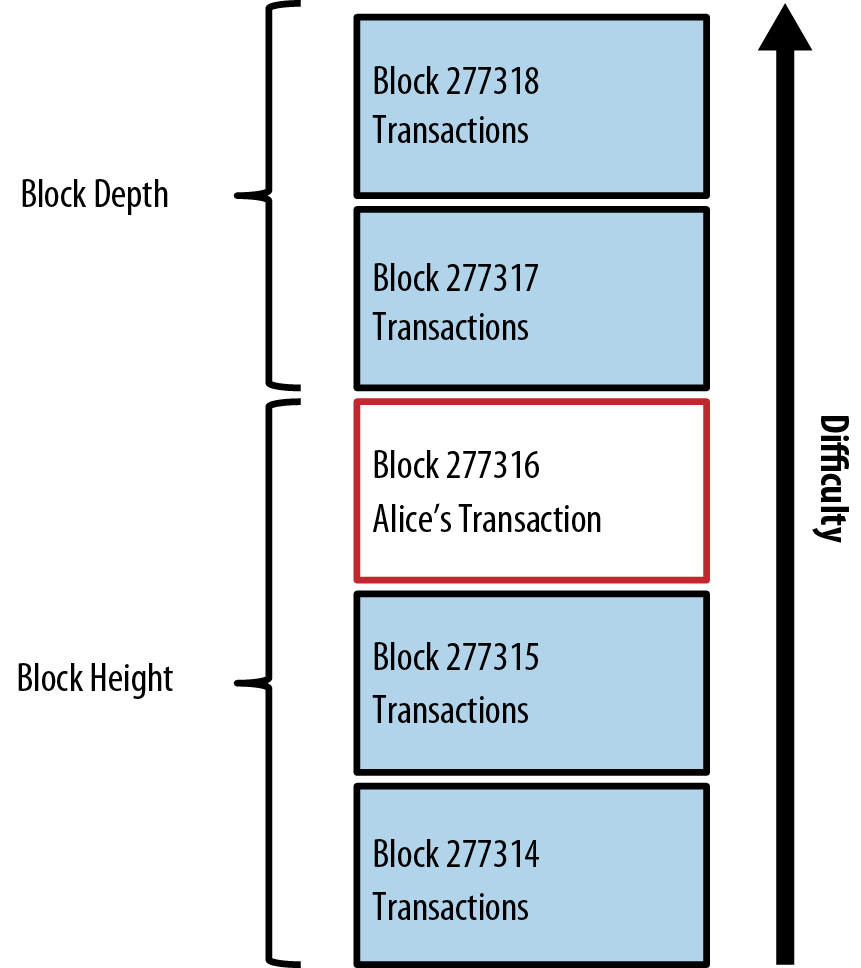
\includegraphics[width=.5\columnwidth]{blockchain-277316} 
	\caption[Transazionte di Alice inclusa nel blocco \texttt{\#277316}]{Transazionte di Alice inclusa nel blocco \texttt{\#277316}}
	\label{fig:blockchain-277316} 
\end{figure}
Da questo punto in poi la transazione di Alice è stata inclusa nella blockchain e sarà visibile a tutte le applicazioni bitcoin. Ogni client bitcoin può verificare indipendentemente la transazione come valida e spendibile. Sarà in oltre possibile tracciare a ritroso il percorso completo del denaro fino alla fonte.

\section{Chiavi, Indirizzi e Wallet}
La proprietà dei bitcoin si stabilisce attraverso chiavi digitali, indirizzi bitcoin e firme digitali. Le chiavi digitali sono create e mantenuti dai vari utenti in un file o database chiamato wallet. Le chiavi digitali nel wallet di un utente sono completamente indipendenti dal protocollo bitcoin e possono essere generate e gestite dal software del wallet dell’utente senza alcuna relazione con la blockchain o accesso a Internet. Esse consentono molte delle interessanti proprietà dei bitcoin, incluso controllo e fiducia de-centralizzata.

Ogni transazione bitcoin richiede una firma valida per essere inclusa nella blockchain, che può essere generata solo con chiavi digitali valide; pertanto, chiunque disponesse di una copia di quelle chiavi ha il controllo del bitcoin in quel conto. Si tratta di coppie di chiavi composte da una chiave privata, che deve rimanere segreta, e una chiave pubblica. Sono in genere memorizzate all'interno del file del wallet e vengono gestite dal relativo software. 

Nella parte di pagamento di una transazione bitcoin, la chiave pubblica del destinatario è rappresentata dalla sua impronta digitale, chiamata indirizzo bitcoin, che viene utilizzata allo stesso modo del nome del beneficiario su un assegno. Nella maggior parte dei casi, un indirizzo bitcoin generato corrisponde ad una chiave pubblica. Tuttavia, non tutti gli indirizzi bitcoin rappresentano chiavi pubbliche; possono anche rappresentare altri beneficiari come gli script, che vedremo più avanti.

\subsection{La Crittografia a Chiave Pubblica e le Criptovalute}
La crittografia a chiave pubblica è stata inventata negli anni '70 (1970) ed è una delle basi matematiche dei computer e della sicurezza informatica.
Da quando stata inventata la crittografia a chiave pubblica, sono state scoperte diverse funzioni matematiche idonee, come ad esempio l’elevazione a potenza dei numeri primi e la moltiplicazione a curva ellittica. Queste funzioni matematiche sono praticamente irreversibili, nel senso che sono facili da calcolare in una direzione e risulta essere molto difficili da calcolare nella direzione opposta. Sulla base di queste funzioni matematiche, la crittografia consente la creazione di segreti digitali e firme digitali non falsificabili. Bitcoin usa la moltiplicazione a curva ellittica come base per la sua crittografia a chiave pubblica.
In bitcoin, usiamo la crittografia a chiave pubblica per creare una coppia di chiavi che controlla l’accesso ai bitcoin. La coppia di chiavi consiste di una chiave privata e un’unica chiave pubblica, l'una derivata dall'altra. La chiave pubblica è usata per ricevere bitcoin, e la chiave privata è usata per autorizzare transazioni per spenderli. C’è una relazione matematica tra la chiave pubblica e quella privata che permette alla chiave privata di essere usata per generare firme sui messaggi. Questa firma può essere validata attraverso la chiave pubblica senza rivelare la chiave privata.
Nella maggior parte delle implementazioni di wallet, le chiavi privata e pubblica sono
salvate insieme come coppia di chiavi per convenienza. Comunque, la chiave pubblica
può essere ricavata dalla chiave privata, quindi è possibile salvare anche solo la
chiave privata.
Un portafoglio bitcoin contiene una raccolta di coppie di chiavi, ognuno composto da una chiave privata e una chiave pubblica. Vediamo come vengono generate queste chiavi:
\begin{itemize}
	\item La chiave privata (k) è un numero, di solito scelto a caso.
	\item Dalla chiave privata, viene utilizzata la curva ellittica, una funzione di crittografia unidirezionale, per generare una chiave pubblica (K).
	\item Dalla chiave pubblica (K), viene utilizzata una funzione di hash crittografica unidirezionale per generare un indirizzo bitcoin (A).
\end{itemize}
La rappresentazione grafica di tutto questo lo si può vedere in Figura \ref{fig:pk-sk-indirizzo-bitcoin}.
\begin{figure}
	\centering 
	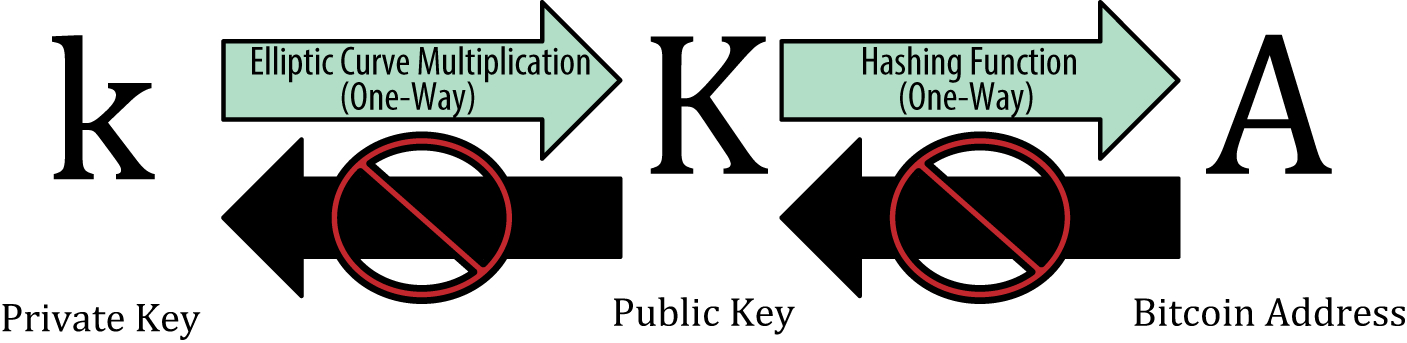
\includegraphics[width=1\columnwidth]{pk-sk-indirizzo-bitcoin} 
	\caption[Chiave privata, chiave pubblica e indirizzo bitcoin]{Chiave privata, chiave pubblica e indirizzo bitcoin}
	\label{fig:pk-sk-indirizzo-bitcoin} 
\end{figure}

\subsubsection{Le chiavi private}
Come abbiamo visto poco fa, una chiave privata è semplicemente un numero scelto casualmente. E' utilizzata per creare le firme necessarie per trasferire i bitcoin, con lo scopo di dimostrare la proprietà dei fondi utilizzati nella transazione. La chiave privata deve essere:
\begin{itemize}
	\item \textbf{Segreta:} rivelarla a terzi equivarrebbe a dare loro il controllo dei bitcoin associati a tale chiave.
	\item \textbf{Protetta da perdite:} deve infatti essere conservata e protetta da perdite accidentali, se questo accadesse i fondi associati ad essa saranno anch'essi persi per sempre.
\end{itemize}
Il primo e più importante passo per generare chiavi è quello di trovare una fonte sicura di entropia, scegli un numero tra $1$ e $2^{256}$. Il metodo utilizzato per la selezione di tale numero non risulta importante fintanto che non sia prevedibile. Il software attuale utilizza il generatore di numeri casuali fornito dall'OS inizializzato però da una fonte esterna di casualità. Più precisamente, la chiave privata potrebbe essere un qualsiasi numero tra $1$ e $n-1$, dove $n$ è una costante ($n=1.158*10^{77}$, un po' meno di $2^{256}$), definito come ordine di curvatura della curva ellittica usata in bitcoin. Si sceglierà un numero casuale di 256 bit inferiore di $n-1$. Questo avviene eseguendo l'algoritmo SHA256 su di una stringa casuale $s$ dove $|s|>256$ bit, questo produrrà comunque un numero di 256 bit. Se tale numero risulterà inferiore di $n-1$ verrà accettato, altrimenti si ripeterà l'algoritmo con un input diverso. La seguente è una chiave privata casuale $k$ mostrata nella sua rappresentazione esadecimale (256 cifre mostrate come 64 cifre esadecimali, ognuna da 4 bit):
\[\text{\small 1E99423A4ED27608A15A2616A2B0E9E52CED330AC530EDCC32C8FFC6A526AEDD}\]
Per generare una nuova chiave tramite il client Bitcoin Core, si utilizza il comando $getnewaddress$. Per ragioni di sicurezza verrà mostrata solamente la chiave pubblica. E' comunque possibile chiedere a Bitcoin Core  di esporre anche le chiave privata tramite il comando $dumpprivkey$ che la mostrerà in formato Base58 checksum-encoded chiamato anche \textit{Wallet Import Format} (WIF).
\begin{lstlisting}
$ bitcoind getnewaddress
 1J7mdg5rbQyUHENYdx39WVWK7fsLpEoXZy
$ bitcoind dumpprivkey 1J7mdg5rbQyUHENYdx39WVWK7fsLpEoXZy
 KxFC1jmwwCoACiCAWZ3eXa96mBM6tb3TYzGmf6YwgdGWZgawvrtJ
\end{lstlisting}
\texttt{NB:} Il comando \textit{dumpprivkey} non genera una chiave privata da una chiave pubblica, visto che è impossibile. Il comando semplicemente rivela la chiave privata che è già conosciuta al wallet e che è stata generata dal comando \textit{getnewaddress}.

\subsubsection{Le chiavi pubbliche}
La chiave pubblica è calcolata da quella privata utilizzando la proprietà di moltiplicazione delle curve ellittiche, operazione irreversibile: $K=k*G$ dove $k$ è la chiave privata, $G$ è un punto costante della curva ellittica chiamato \textit{Generator Point} e $K$ sarà la chiave pubblica risultante. L'operazione inversa, conosciuta come trovare il logaritmo discreto, calcolando $k$ conoscendo $K$, risulta difficile come provare per tutti i possibili valori di $k$, brute-force search.

\subsubsection{Crittografia e Curve Ellittiche}
Le curve ellittiche in crittografia sono un tipo di crittografia assimmetrica, utilizzano coppie di chiavi $(Pk, Sk)$, basata sul problema del logaritmo discreto. La curva utilizzata da bitcoin è definita in uno standard detto \textit{secp256k1} dal National Institute of Standards and Technology (NIST). La \textit{secp256k1} è definita dalla seguente funzione:
\[  y^{2}=(x^{3}+7) \text{ over } (\mathbb{F}_{p}) \quad \text{ or } \quad y^{2} \bmod p=(x^{3}+7) \bmod p\]
Il $\bmod p$ indica che questa curva è su di un campo finito di numeri primi di ordine $p$, ch possiamo definire come $\mathbb{F}_{p}$ dove $p = 2^{256} - 2^{32} - 2^{9} - 2^{8} - 2^{7} - 2^{6} - 2^{4} - 1$, in parole povere, un numero primo molto grande.
Nella matemetica delle curve ellittiche c'è un punto chiamato \textit{point as infinity}, il quale viene fatto corrispondere allo zero nell'addizione.
Esiste un operatore $+$, chiamato addizione che dati due punti $P_{1}$ e $P_{2}$ sulla curva ellittica, $\exists P_{3} \quad | \quad P_{3} = P_{1} + P_{2}$. Geometricamente, questo nuovo punto $P_{3}$ viene calcolato tracciando una linea tra $P_{1}$ e $P_{2}$. Questa linea intersecherà la curva ellittica nel punto addizionale chiamato appunto $P_{3} = (x, y)$. Tale punto lo possiamo riflettere sull'asse delle $x$ ottenendo $P_{3} = (x, -y)$. Esistono vari casi particolari di queste addizioni tra punti, se il lettore ne fosse interessato è consigliata la lettura dei testi \cite{mastering:andreas} e \cite{mastering2:andreas}.

\subsubsection{Generazione della chiave pubblica}
Partendo da una chiave privata $k$, numero generato casualmente, lo moltiplichiamo con un punto predeterminato sulla curva, denominato \textit{generator point} $G$ producendo un ulteriore punto situato in qualche altra parte della curva. Questo punto sarà la chiave pubblica $K$. 
\[ K=k*G\]
Poiché il punto di generazione $G$ è sempre lo stesso per tutti gli utenti di bitcoin, una chiave privata $k$ moltiplicata per $G$ darà sempre come risultato la stessa chiave pubblica $K$. La relazione tra $k$ e $K$ è fissa, ma può essere calcolata in una sola direzione.
\[ k \Rightarrow K \quad k \nLeftarrow K\]
Per questo motivo la chiave pubblica, $K$, di un utente può essere condivisa con chiunque senza rivelare alcuna informazione circa la relativa chiave privata, $k$.
Moltiplicare $G$ per un qualsiasi numero $k$ equivale ad aggiungere $G$ a se stesso $k$ volte di seguito. Nelle curve ellittiche, aggiungere un punto a se stesso equivale a tracciare una linea tangente al punto e trovare quindi dove questa interseca nuovamente la curva, infine riflettiamo questo punto sull'asse delle $x$. La dimostrazione grafica di queste operazioni eseguite in modo consecutivo lo troviamo in Figura \ref{fig:crittografia-ellittica}.
\begin{figure}
	\centering 
	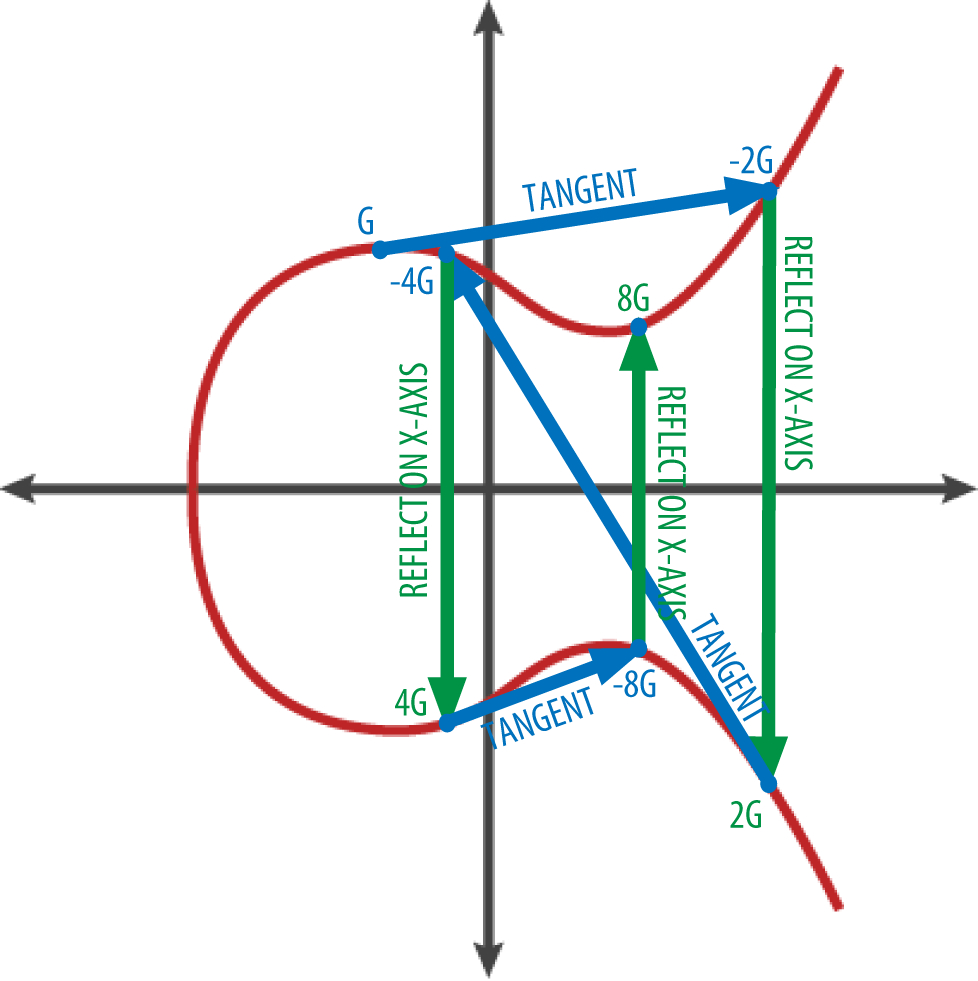
\includegraphics[width=.6\columnwidth]{crittografia-ellittica} 
	\caption[Crittografia Ellittica]{Schema di funzionamento della moltiplicazione nelle curve ellittiche, $G*k$.}
	\label{fig:crittografia-ellittica} 
\end{figure}

\subsubsection{Indirizzi Bitcoin}
Un indirizzo bitcoin è una stringa di cifre e caratteri che può essere condivisa con chiunque desideri inviarti denaro. Gli indirizzi prodotti dalle chiavi pubbliche sono costituiti da una stringa di numeri e lettere che inizia con $1$. Ecco un esempio di indirizzo bitcoin:
\[ \text{1J7mdg5rbQyUHENYdx39WVWK7fsLpEoXZy} \]
Questo indirizzo è quello che appare comunemente in una transazione come \textit{destinatario} dei fondi. Un indirizzo bitcoin può rappresentare un proprietario di una coppia di chiavi $(Pk,Sk)$, oppure qualcos'altro come uno script di pagamento. 
L'indirizzo bitcoin è derivato dalla chiave pubblica attraverso l'uso di una funzione one-way\footnote{Una funzione one-way è una funzione matematica unidirezionale cioè "facile da calcolare", ma "difficile da invertire"} in questo caso un hashing crittografico. tali funzioni sono usate ampiamente in bitcoin: negli indirizzi bitcoin, negli indirizzi di script e negli algoritmi di \textit{proof-of-work}. Gli algoritmi utilizzato sono in particolare:
\begin{description}
	\item[SHA] (Secure Hash Algorithm) in particolare SHA256.
	\item[RIPEMD] (RACE Integrity Primitives Evaluation Message Digest) in particolare RIPEMD160.
\end{description}
Iniziando dalla chiava pubblica $K$, ne calcoliamo l'hash \textit{SHA256} e successivamente l'hash \textit{RIPEMD160}, producendo un numero a 160 bit (20 byte) chiamato $A$. La rappresentazione grafica di queste fasi la si può vedere in Figura \ref{fig:pk-to-indirizzo-bitcoin}.\\
\texttt{NB:} l'indirizzo bitcoin non è la chiave pubblica. Gli indirizzi bitcoin sono derivati da una chiave pubblica utilizzando una funzione one-way come abbiamo appena visto. Gli indirizzi bitcoin sono quasi sempre presentati agli utenti in una codifica chiamata \textit{Base58Check} che utilizza 58 caratteri ed un checksum per facilitarne la lettura evitando ambiguità proteggendo l'utilizzatore da errori di trascrizione.
\begin{figure}
	\centering 
	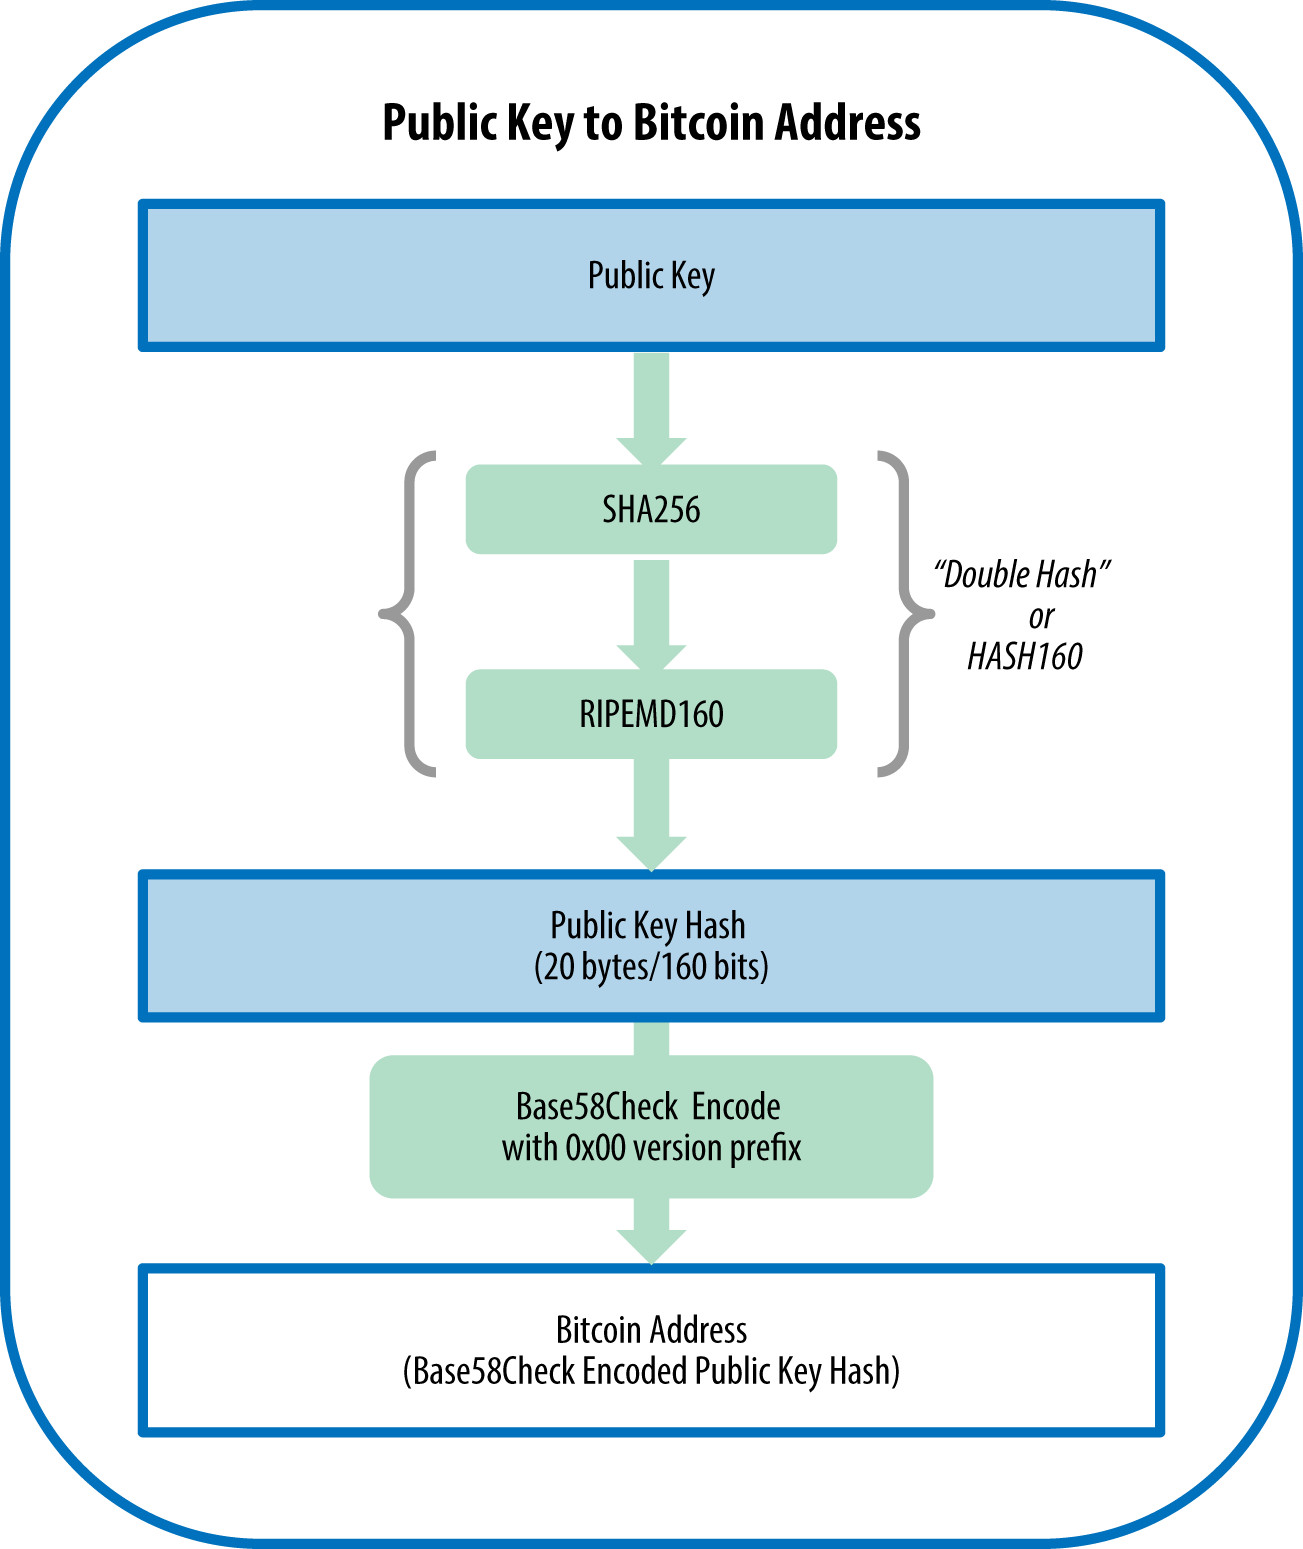
\includegraphics[width=.6\columnwidth]{pk-to-indirizzo-bitcoin} 
	\caption[Da chiave pubblica a indirizzo bitcoin]{Conversione di una chiave pubblica in un indirizzo bitcoin}
	\label{fig:pk-to-indirizzo-bitcoin} 
\end{figure}

\subsection*{I Wallet}
I wallet sono dei contenitori di chiavi private, non monete, solitamente implementati come file strutturati o semplici database. Gli utenti firmano le transazioni con queste chiavi, dimostrando di possedere gli output delle transazioni precedenti, utilizzati come input per le nuove transazioni. La valuta (bitcoin) è memorizzata sulla blockchain sotto forma di transazioni di output.
\subsubsection{Wallet non deterministici}
Nei primi client bitcoin, i wallet erano semplicemente delle raccolte di chiavi private generate casualmente. Questo tipo di portafoglio è chiamato \textit{Type-0 nondeterministic wallet}, sono soprannominati \textit{"Just a Bunch Of Keys"} o JBOK, sono stati sostituiti dai wallet deterministici poiché scomodi da gestire. La scomodità di un wallet non deterministico sta nel fatto che si è obbligati ad eseguire molto spesso dei backup di tutte queste, dato che il loro smarrimento implica la perdita della valuta in bitcoin a cui sono legate. Dato che il riutilizzo degli indirizzi riduce la privacy, si è portati ad una continua generazione di nuove chiavi quindi, per sicurezza, si dovrà rieseguire il backup. Nonostante Bitcoin Core includa un portafoglio di tipo zero, il suo utilizzo è sconsigliato dato che c'è la possibilità di utilizzare un wallet di tipo deterministico. Vedi Figura \ref*{fig:wallet-non-deterministico}.

\subsubsection{Wallet deterministici}
I wallet deterministici sono stati sviluppati per consentire di derivare chiavi multiple da un singolo seme \textit{seed}. La forma più avanzata di questo tipo di wallet è il \textit{hierarchical deterministic wallet} o \textit{HD wallet} definito dallo standard \texttt{BIP0032}, come dice il nome, contengono chiavi derivate in una struttura ad albero tale per cui da ogni chiave madre si possa derivare una sequenza di chiavi figlie e per ognuna di esse si possa derivare una sequenza di chiavi nipote ecc \dots ad una profondità infinita. Tale struttura la possiamo vedere in Figura \ref{fig:wallet-deterministico}
\begin{figure}
	\centering
	\subfloat[][\emph{Wallet non deterministico}]
	{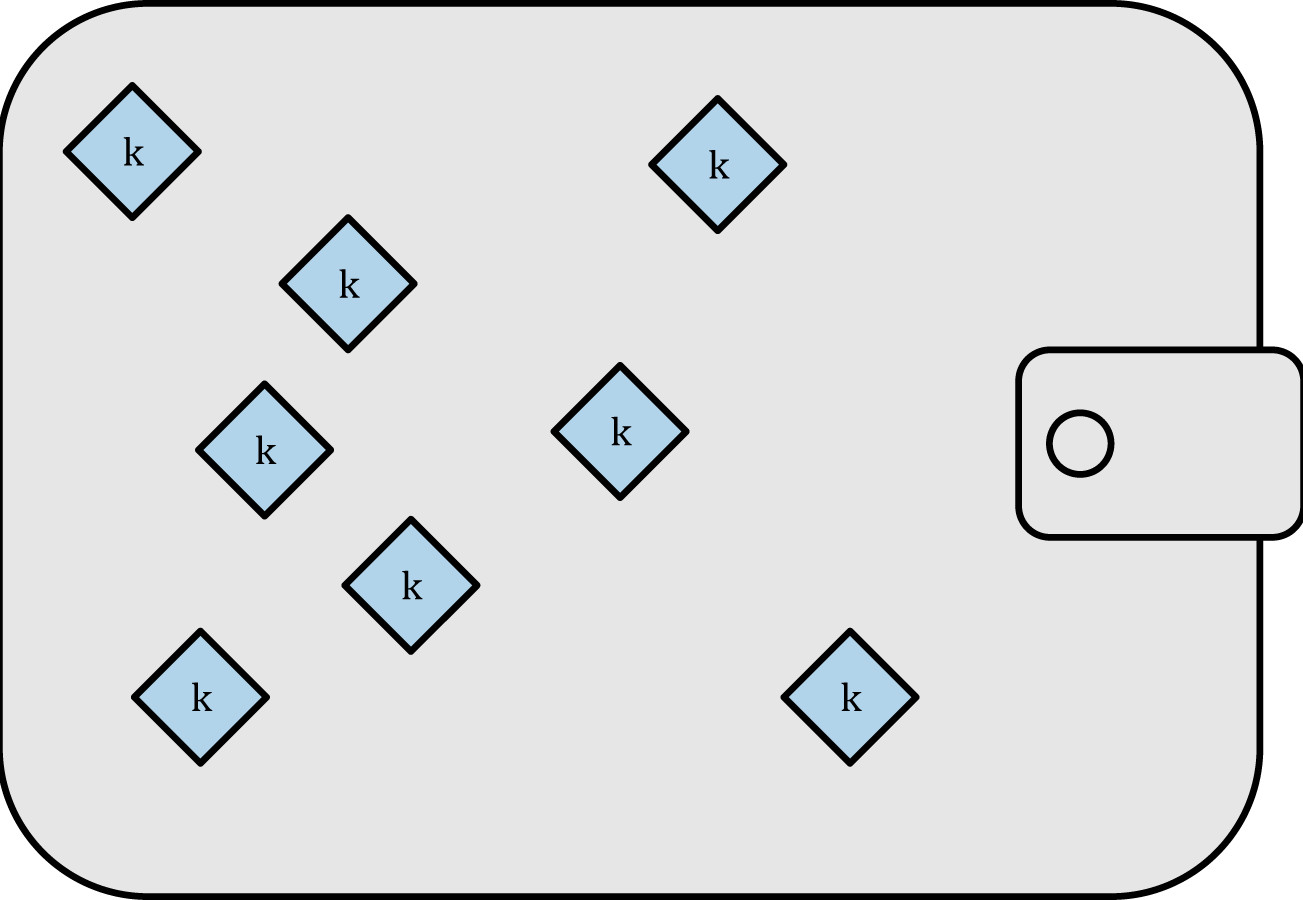
\includegraphics[width=.45\textwidth]{wallet-nondeterministico}
	\label{fig:wallet-non-deterministico}} \quad
	\subfloat[][\emph{Wallet deterministico}]
	{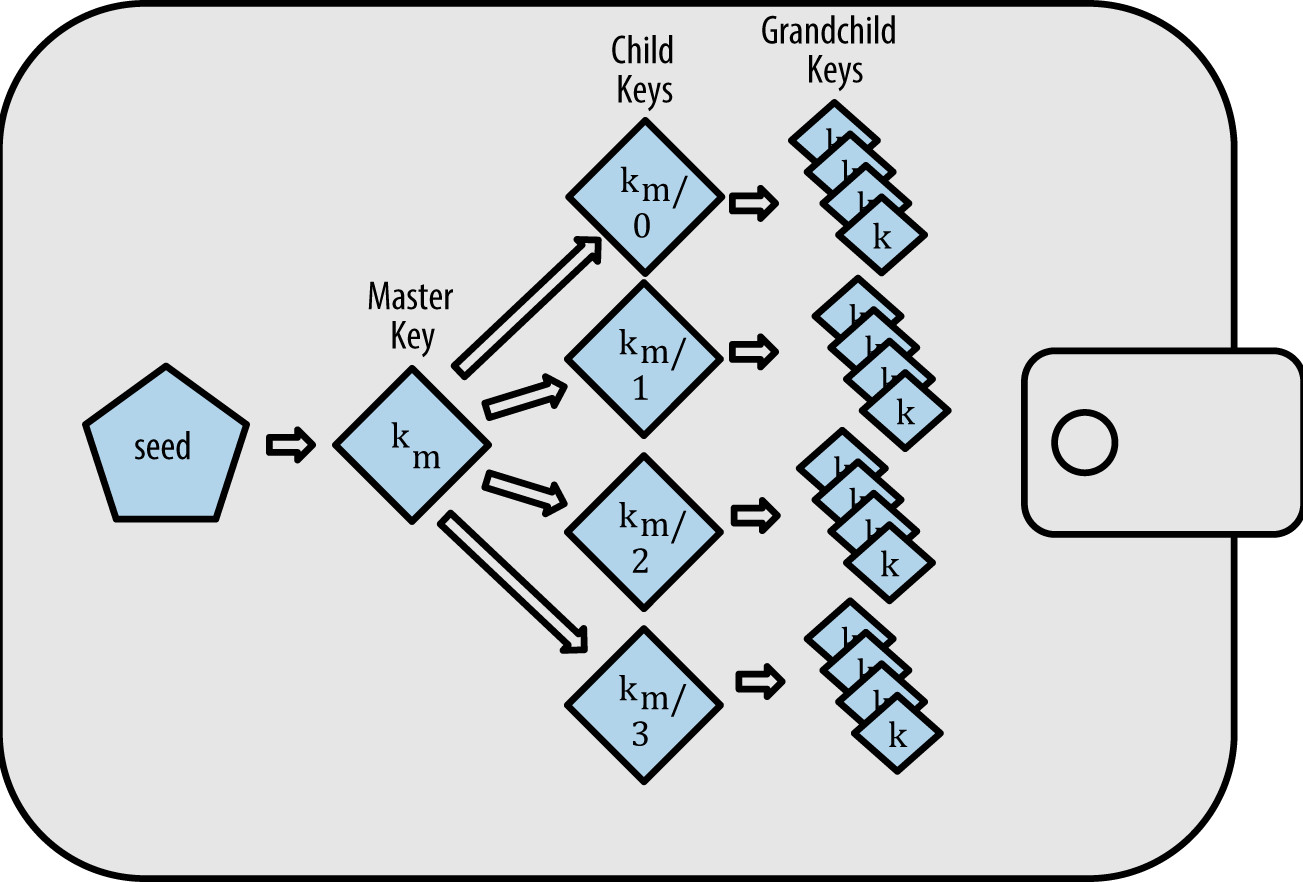
\includegraphics[width=.45\textwidth]{wallet-deterministico}
	\label{fig:wallet-deterministico}}
	\caption{Due tipologie di Wallet}
	\label{fig:tipologie-di-wallet}
\end{figure}
Gli \textit{HD wallet} offrono due importanti vantaggi rispetto alle chiavi casuali.
\begin{itemize}
	\item La struttura ad albero può essere utilizzata per rappresentare una struttura organizzativa aggiuntiva, per esempio alcuni rami potrebbero essere utilizzati per generare chiavi impiegate poi in diversi settori aziendali.
	\item Gli utenti possono creare sequenze di chiavi pubbliche $K_{i}$ senza avere accesso alle corrispettive chiavi private. Questo permette di utilizzare gli HD wallet anche su di un server non sicuro che riuscirà ad emettere una diversa chiave pubblica per ogni transazione.
\end{itemize}

\subsubsection{Vanity Address}
I vanity address sono indirizzi bitcoin validi che contengono dei messaggi mnemonici con un significato per l'uomo. Per esempio \texttt{1LoveBPzzD72PUXLzCkYAtGFYmK5vYNR33} è uno di questi in cui notiamo la presenza della parola \texttt{Love} all'inizio dell'indirizzo. Il processo consiste essenzialmente nel selezionare una chiave privata a caso,derivando la chiave pubblica, derivando l’indirizzo bitcoin e verificando se corrisponde al modello di vanità desiderato, ripetendo miliardi di volte fino a che non verrà trovata una corrispondenza. Questa tipologia di indirizzi non sono più sicuri di qualsiasi altro indirizzo, dipendono dalla stessa Elliptic Curve Cryptography (ECC) e Secure Hash Algorithm (SHA) come qualsiasi altro indirizzo.
\begin{table}[]
	\centering
	\begin{tabular}{|c|c|c|c|c|}
		\hline
		\textbf{Dim.} 	& \textbf{Pattern} 	& \textbf{Frequenza} 		& \textbf{Tempo medio} \\ \hline
		1 			& 1K 		& 1 su 58 chiavi 	& < 1 millisecondi \\ \hline
		2 			& 1Ki 		& 1 su 3,364 		& 50 millisecondi \\ \hline
		3 			& 1Kid 		& 1 su 195,000 		& < 2 secondi \\ \hline
		4 			& 1Kids 	& 1 su 11 million 	& 1 minuto \\ \hline
		5 			& 1KidsC 	& 1 su 656 milioni 	& 1 ora \\ \hline
		6 			& 1KidsCh 	& 1 su 38 miliardi 	& 2 giorni \\ \hline
		7 			& 1KidsCha 	& 1 su 2.2 mila miliardi 	& 3–4 mesi \\ \hline
		8 			& 1KidsChar & 1 su 128 mila miliardi 	& 13–18 anni \\ \hline
		9 			& 1KidsChari 	& 1 su 7 milioni di miliardi	& 800 anni \\ \hline
		10 			& 1KidsCharit 	& 1 su 400 milioni di miliardi	& 46,000 anni \\ \hline
		11 			& 1KidsCharity 	& 1 su 23 mila milioni di miliardi	& 2.5 milioni di anni \\ \hline
	\end{tabular}
	\caption{Frequenza del vanity pattern \textit{1KidsCharity} e relativo tempo di ricerca su di un medio PC fisso.}
	\label{tab:vanity-address-table}
\end{table}
Generare un vanity address è un esercizio di forza bruta, come riportato in Tabella \ref{tab:vanity-address-table}, notiamo che più grande è il pattern che desideriamo sia presente all'inizio dell'indirizzo, più difficile sarà trovarlo quindi necessiterà di più tempo computazionale. 

Questi indirizzi possono essere utilizzati per migliorare o adirrittura sconfiggere la sicurezza, sono infatti un'arma a doppio taglio, vediamo perché:
\begin{itemize}
	\item \textbf{Migliora la sicurezza:} un indirizzo distintivo rende più difficile per gli avversari sostituire il proprio indirizzo e ingannare i clienti reindirizzando i fondi.
	\item \textbf{Ingannevoli:} sfortunatamente è possibile a chiunque creare un vanity address fraudolento che assomigli a qualsiasi altro indirizzo casuale, riuscendo ad ingannare i clienti altrui.
\end{itemize}
L'idea è far generare un vanity address da una vanity pool riuscendo quindi a cercare un indirizzo con un pattern abbastanza lungo, per esempio 8 caratteri. Un attaccante che intende ingannane gli utilizzatori di tale indirizzo tenteranno di aggiungere ulteriori caratteri al pattern, facendoli combaciare con quelli dell'indirizzo originale. Questa operazione implica un costo aggiuntivo per l'attaccante, se il bottino ottenibile dalla frode non fosse abbastanza alto da coprire il costo della generazione dei tale indirizzo fraudolento di vanità.

\subsection{La rete bitcoin}
Bitcoin è strutturato come un'architettura peer-to-peer, ciò sta a significare che i computer, nodi, che partecipano alla rete sono tutti alla pari, non ci sono nodi speciali e tutti loro condividono il compito di fornire servizio alla rete. Non esiste infatti un server o servizio centralizzato o gerarchia di qualunque tipo.

\subsubsection{Tipologie di Nodi e Ruoli}
Nonostante tutti i nodi della rete P2P bitcoin siano uguali, possono avere differenti ruoli a seconda della funzionalità che stanno supportando. Un nodo bitcoin è una serie di funzioni: routing, database della blockchain, mining, e servizi wallet, un nodo con tutte queste funzioni è appunto chiamato \textit{full-node}. Un esempio di network eterogeneo lo si può vedere in figura \ref{fig:network-bitcoin}.
\begin{figure}
	\centering 
	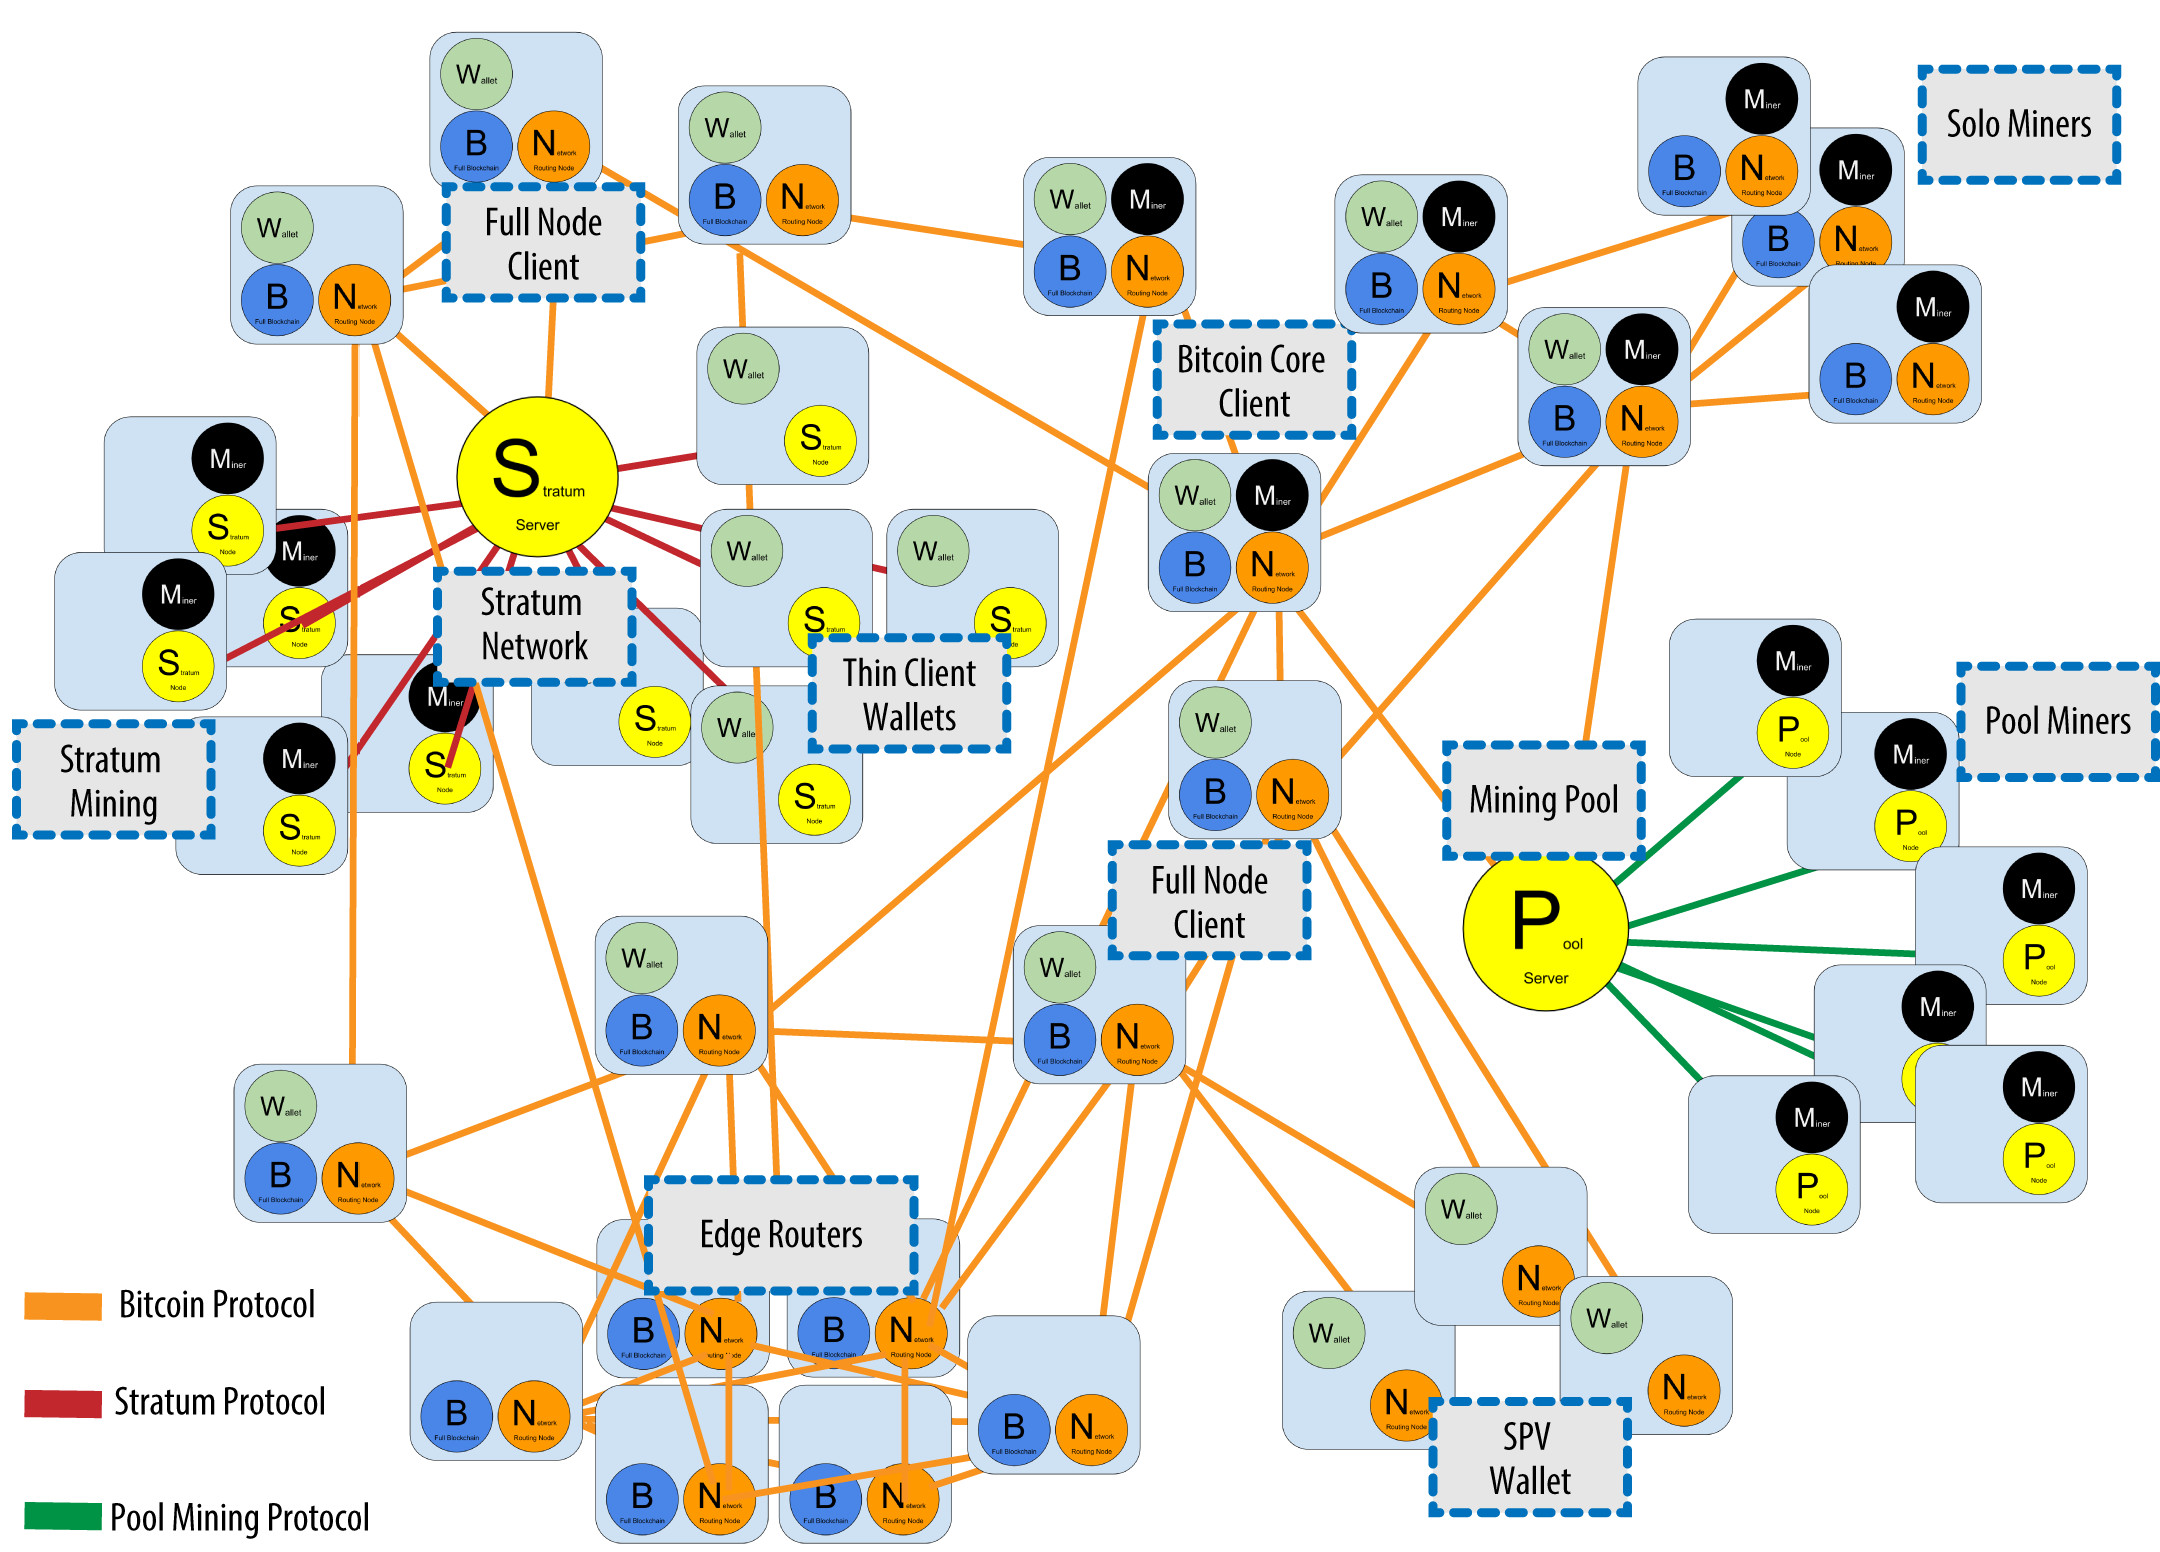
\includegraphics[width=1\columnwidth]{network-bitcoin} 
	\caption[Network bitcoin]{Rete estesa di bitcoin con vari tipologie di nodi, gateway e protocolli.}
	\label{fig:network-bitcoin} 
\end{figure}

\section{Blockchain}
La struttura dati blockchain risulta un'ordinata lista di blocchi contenenti transazioni back-linked\footnote{blocchi sono collegati a ritroso, ognuno si riferisce al blocco precedente presente nella catena}. La blockchain è spesso visualizzata come una pila verticale, con blocchi stratificati l’uno sopra l’altro e il primo blocco serve da fondamenta della pila. La visualizzazione dei blocchi impilati uno sopra l’altro provoca l’uso di terminologie come "altezza" (height) per riferirsi alla distanza dal primo blocco, e \textit{top} per riferirsi al blocco aggiunto più recentemente. Anche se un blocco ha solo un genitore, può temporaneamente avere multipli figli. Ognuno dei figli si riferisce allo stesso blocco del padre e contiene lo stesso hash (padre) nel campo \textit{previous block hash}. Multipli figli emergono durante un fork della blockchain, una situazione temporanea che accade quando differenti blocchi sono scoperti quasi simultaneamente da miner differenti. In questo caso solo un blocco figlio diventa parte della blockchain i il fork viene quindi risolto. Il campo \textit{previous block hash} risulta molto importante al fine di rendere le transazioni passate sempre più affidabili, tale campo infatti è incluso nell'header del blocco e per questo motivo influenza l'hash del blocco attuale. La modifica di una transazione all'interno di un blocco genitore porta alla modifica del proprio hash che di conseguenza porta alla modifica dell'hash figlio, questo fino al vertice della blockchain. Visto che per questo ricalcolo servirebbe un’enorme
potenza computazionale, l’esistenza di una lunga catena di blocchi fa si che la storia più profonda della blockchain sia immutabile, che è uno degli elementi chiave della sicurezza di bitcoin.
\begin{table}[]
	\centering
	\begin{tabular}{|c|c|p{6cm}|}
		\hline
		\textbf{Dim.} 		&	\textbf{Campo} 					& \textbf{Descrizione} \\ \hline
		4 byte						& Versione 							& Un numero di versione per tracciare upgrade al software e/o al protocollo \\ \hline
		32 byte 					& Hash del Blocco Precedente 		& Un riferimento all’hash del blocco precedente \\ \hline
		32 byte 					& Merkle Root 						& Un’hash della radice del merkle tree delle transazioni di questo blocco \\ \hline
		4 byte 						& Timestamp 						& Il tempo approssimato della creazione del blocco corrente (Unix Epoch)\\ \hline
		4 bytes 					& Target di Difficoltà				& Taghet di difficoltà dell’algoritmo di proof-of-work per questo blocco \\ \hline
		4 byte 						& Nonce 							& Un contatore utilizzato per l’algoritmo di proof-of-work\\ \hline
	\end{tabular}
	\caption{La struttura di un block header}
	\label{tab:struttura-block-header}
\end{table}
Nella Tabella \ref{tab:struttura-block-header} troviamo indicato anche \textit{Markle Root}, conosciuto anche come un \textit{binary hash tree}, è una struttura dati usata per indicizzare efficientemente e verificare l’integrità di un grande gruppo di dati. Sono usati in bitcoin per indicizzare tutte le transazioni in un blocco, producendo in sostanza un’impronta digitale dell’intero set di transazioni, provvedendo ad un efficiente processo di verifica se una transazione è inclusa nel blocco. 

\subsubsection{Target di difficoltà}
Il target determina la difficoltà e quindi influenza il tempo necessario per trovare una soluzione da parte dell'algoritmo \textit{proof-of-work}. Come sappiamo i bitcoin vengono generati ogni 10 minuti circa questo è il battito di emissione della valuta che deve rimanere costante negli anni. Col passare degli anni si avrà un rapido aumento della potenza di calcolo degli elaboratori e inoltre sempre più utenti prenderanno parte alla network bitcoin. Questo comporta che sarà sempre più facile arrivare ad una soluzione proof-of-work, perciò si deve procedere con l'aumento della difficoltà di tale algoritmo al fine di mantenere la generazione di nuovi blocchi fissa a 10 minuti. Questo retargeting avviene in modo automatico su ogni nodo. Ogni 2016 blocchi, tutti i nodi ritarano la difficoltà proof-of-work. L'equazione è semplice, si misura il tempo effettivo impiegato per generare gli ultimo 2016 blocchi e lo si confronta con il tempo atteso di 20160 minuti. 
\[ \text{New Difficulty = Old Difficulty * (Tempo degli ultimi 2016 Blocchi / 20160 min)} \]

\subsection{Fork della blockchain}
La blockchain è una struttura dati decentralizzata e le diverse copie nella network non sono sempre identiche. Come sappiamo la procedura di mining è una competizione globale nel tentativo di arrivare prima ad una soluzione proof-of-work- La velocità con cui l'aggiornamento della blockchain si propaga nella neetwork può far si che in caso due miner trovino due proof-of-work diverse, ma comunque valide, generano all'interno della rete un fork. Questo significa che il penultimo blocco aggiunto ha generato due o più figli. Da questo momento la network bitcoin si divide in sezioni, ognuna lavorerà per cercare di aggiungere un blocco al di sopra del blocco figlio che arrivò per primo. Con molta probabilità un solo altro miner troverà una soluzione che accrescerà una delle due ramificazioni. Da questo momento in poi la blockchain valida per tutti i miner sarà quella con proof-of-work più alto, la catena più lunga. L'effetto di questa scelta andrà ad incidere sul lavoro che altri miner hanno svolto sull'altro ramo della catena. Le transazioni incluse nei blocchi di quel ramo verranno scartate, tranne quelle non incluse nei blocchi dell'attuale catena principale, che verranno rimessi in coda. Un classico fork può capitare ogni settimana ma normalmente vengono risolte dopo il calcolo di un blocco, raramente due miner trovano altre due soluzioni quasi contemporaneamente. La visione grafica degli eventi appena descritti si possono vedere in Figura \ref{fig:fork-blockchain}.
\begin{figure}
	\centering
	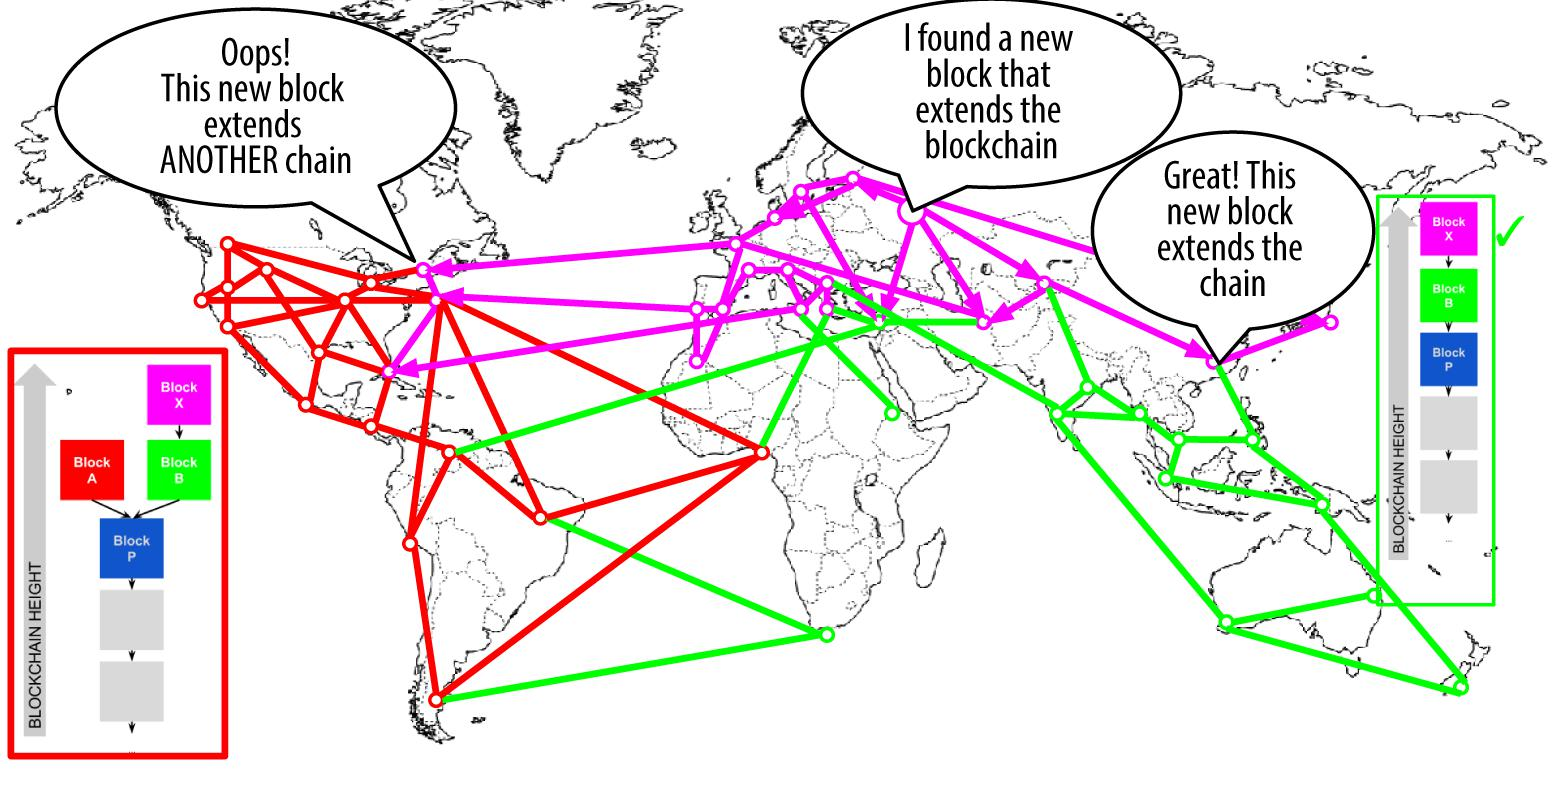
\includegraphics[width=1\linewidth]{Immagini/fork-blockchain}
	\caption[Visualizzazione di un’evento di fork di blockchain]{Visualizzazione di un’evento di fork di blockchain: il network riconverge su di una nuova longest chain}
	\label{fig:fork-blockchain}
\end{figure}

\subsection{Attacchi al consenso}
Il meccanismo di consenso in bitcoin dipende dal fatto che la maggioranza dei miner agisca onestamente, tuttavia se un miner o un gruppo di miner raggiunge una quota significativa del potere di calcolo, essi possono attaccare il meccanismo di consenso in modo da interrompere la sicurezza e la disponibilità della rete bitcoin. Gli attacchi di consenso possono influenzare il futuro e il passato più recente (all'incirca 10 blocchi), andando a forzare eventuali fork secondari della blockchain. Un fork può essere raggiunto da qualsiasi profondità ma nella pratica la potenza di calcolo necessaria per forzare un fork molto profondo risulta essere immensa. Questo rende i blocchi, confermati $n$ volte, praticamente immutabili. Un attacco di questo tipo non può spendere bitcoin senza l'utilizzo di firme, reindirizzare bitcoin o modificare in qualsiasi altro modo le transazioni. Gli attacchi di consenso possono interessare solo i blocchi più recenti e causare denial-of-service sulla creazione di blocchi futuri. Un attacco di questo tipo viene chiamato \textbf{Attacco del 51\%}, in questo scenario un gruppo di miner, controllando il 51\% della potenza di hashing della network bitcoin, hanno la possibilità di portare a termine con successo questo tipo di attacco. Possono causare deliberatamente dei fork, double-spending o eseguire attacchi di denial-of-service contro specifiche transazioni / indirizzi. Nonostante il suo nome, questo tipo di attacco in realtà non richiede il 51\% della potenza di hashing. Tale soglia rappresenta semplicemente il livello al quale l'attacco è quasi sicuramente di successo. Vari gruppi di ricerca, utilizzando degli strumenti statistici, affermano che vari tipi di attacchi di consenso sono possibili utilizzando anche solo il 30\% della potenza di hashing.

\section{Alt-Chain e Alt-Coin}
Bitcoin è il risultato di ben 20 anni di ricerca sui sistemi distribuiti e valute che ha portato ad una tecnologia rivoluzionaria: il meccanismo di consenso decentralizzato basato sulla proof-of-work. Questa invenzione è il cuore di bitcoin e ha successivamente generato un'onda di innovazione in valuta, servizi finanziari, eco	nomia, sistemi distribuiti, sistemi di votazione e contratti. Sono infatti nate delle:
\begin{description}
	\item[Alt-coin] valute digitali implementate utilizzando lo stesso modello di implementazione di bitcoin, la maggior parte delle implementazioni derivano da codice sorgente di bitcoin. Questo tipo di valuta sono chiamate anche \textit{fork} di bitcoin. Poi co sono anche delle alt-coin implementate da zero basate solamente sul modello blockchain ma che non riutilizzano il codice sorgente di bitcoin. Tra le principali troviamo Litecoin, Dogecoin, Freicoin, NXT.
	\item[Alt-chain] blockchain alternative il cui vero scopo non è quello di realizzare un sistema monetario. Queste diverse implementazioni possono comunque includere anche una valuta ma questa viene emessa come token per allocare dell'altro, come una risorsa o un contratto. Tra la principali troviamo Namecoin ed Ethereum.
\end{description}